\todoinline{
    Practical Work
    This is a description and discussion of the practical work you have carried out. You have defined how it is to be assessed in the Terms of Reference.
    How to organise the practical work chapters varies between projects, depending to the nature of your practical work. If you have conducted an investigative work
    without the aid of a product, you should organise the contents into three chapters as Design, Investigation and Results. However, if your practical work is mainly
    the development of a product, it makes more sense that you organise the chapters in terms of the product development life cycle, i.e., Design, Implementation and Testing.
    Please choose from below the appropriate section to read considering the nature of your own project.

    •	Projects focusing on the development of a product
    You should discuss the design, implementation, and testing of your product. There are sections on each of these below. If there were other activities involved in development,
    such as analysis modelling based on the requirements specification, or if your project involved other practical work such as an experiment using your product, you should also
    include these: say what you did and discuss any interesting decisions or problems. If your product does not fit this model - for example, a project whose product is an
    information strategy - this section should discuss the work needed to create that product.

    The narrative should especially identify areas of the work that were particularly interesting or difficult. Assume that the readership of the report will be computer
    literate individuals who will appreciate the problems you have tackled.
    Justify in detail the method(s) you chose to synthesise a solution to the problem. Discuss how your reading of the literature guided you in your work. You may wish to
    refer to supporting documentation in your discussion of the solution; these will be held in appendices to the report.
    In general, there should be neither bookwork nor theoretical material here. You should tell the reader what you did, why you did it and how you did it. Unless you have
    developed a worthwhile product or solved a challenging problem there will be little for you to say (and few marks to gain).
}

\section{Design}
\todoinline{
    Good products, whether software or hardware, must be designed. It is not professional to hack out a solution! You must describe and provide a rationale for that design.
    The artefacts produced are models (and perhaps prototypes) that form part of your product. In the report you tell the reader about your design and discuss the design
    decisions. Throughout the design section you should justify your choices. Discuss the implications of making different design choices, and the reasons for the design
    that you have selected.

    The design chapter(s) should give a top-level view of how your product meets its requirements. For a software product, a good starting point is to describe the architecture
    of the software. (If your product is not software, what corresponds to the software architecture?)  For example, suppose you are going to produce a computer game that
    could be played across the web. This will involve some software concerned with the communications across the network, some software concerned with the specific game and
    some with aspects that could be common to many games. This suggests an architecture consisting of three subsystems. You may feel there are other possible designs. If so,
    discuss each and then tell the reader which you decided to follow, and why.

    Once you have selected a top-level design you can start to look at the details of each product component. You will produce design models as required by the development
    approach that you are following, and you will need to discuss your design decisions. For example, if you are using an object-oriented approach, you will probably describe
    and justify the important classes in your system. Design patterns are an area of increasing popularity and usefulness. Investigate making use of some. Explain which you
    have used and why.

    Make careful use of figures and diagrams when describing the design. Any diagrams are there to help the reader understand what you have done. They must form a minor
    part of the chapter. The full design documentation will be marked under the product marking part of the module.
    Another aspect of the design, which you may wish to write about, is the user interface. There is no point in simply relating HCI theory here, and merely describing
    or giving pictures of your screen designs is also inadequate: what the reader wants to know is how you have applied the theory. Justify your design choices in terms of
    usability principles, and illustrate them with a few carefully selected screen dumps.

    You may wish to discuss the design process that you followed. Theoretical descriptions of design processes are unlikely to be interesting here. How you applied the
    process and how it affected your product, might be.
}

\todo{Design}

\section{Implementation}

\todoinline{
    In an implementation chapter, you are describing and justifying how you implemented your product, which for a software product means at the code level.
    Do not attempt to describe every detail. For a software product, do not include large sections of program code. Any code presented should be to illustrate important
    and interesting features. You might want to describe the data structures you elected to use, e.g. in Java a LinkedList or a Vector, and explain why you chose the one
    you did. If there were any interesting low-level algorithms, you should describe these. If you feel it is important to put a significant volume of program code into
    your report, put it in an appendix and reference the appendix. (The appendix usually contains examples of your code, but the place for your full code is in your OneDrive
    product folder.)

    Writing about program code can sometimes cause a student problems. You should be able to find good examples of articles that discuss implementations on the web.
    Read them and learn from how they do it. For Java a good source of examples can be found at JavaWorld.com.
    Pick out the key parts of your implementation and provide a rationale for them. During your attempts to implement your product, you may have had to face unforeseen
    problems. Explain how you overcame them. They may have caused you to modify the original design. Discuss the implications of those changes.
}

\todo{Implementation}

The \chef{} app is implemented using a React frontend and an Express.js backend, both written in TypeScript.
This language was chosen as it compiles into JavaScript that can run in a browser, allowing the same language to be used for both
the front and back ends, while adding compile-time type checking similar to strongly typed languages such as Java.

\section{Backend Implementation}
\todo{Backend}

The backend of the app is implemented as a REST API based on Express.js with SQLite
used for the database.

\todo{Expressjs}

SQLite was chosen for the database as it is the simplest to set up, being implemented through
a library rather than requiring a dedicated server, while being somewhat portable with other
database systems.~\cite{kreibich_using_2010} This would allow for the database to be migrated to
another backend with a limited number of changes needing to be made.

One major difference between TypeScript and Java is that TypeScript uses structural typing, where objects are considered
the same if they have the same structure. While Java uses nominal typing and requrires an interface to be explicitly
implemented by a class. This allows for different modules to be interoperable through sharing the same structure of objects.~\cite{gil_whiteoak_2008}
For this reason, along with the fact that the data transfer objects did not need their own logic, it was decided early on
to not use classes for objects retrieved from the database and instead to rely on interfaces only.


\subsection{Documentation}
The API was declared and documented using the OpenAPI format and converted
into TypeScript types using the \codelisting{openapi-typescript} package. These
generated types were then used to check the return types from the API.

The \codelisting{express-openapi-validator} package was used separately to validate
request parameters against the OpenAPI schema. This implementation avoided having
to duplicate validation specificiations and removed the possibility of having the values that
the server accepts differ from what was documented.

One limitation that was not resolved with either of the above packages is that there is no validation
for whether the endpoints exist which lead to some confusion when testing endpoints that had not been registered
with Express. A different combination of packages may have been able to check for this,
but was not considered due to time constraints.

Swagger UI \cite{smartbear_swagger_2024} was used to serve a generated HTML page that lists all endpoints declared in
the API specification, along with example values for both requests and responses and the ability to make requests in
the browser. This served as a quick way to make test requests with dummy data during development, and an easy-to-use
reference for the endpoints available to \codelisting{openapi-fetch}.

\subsection{Machine Learning}
The similarity of recipes is evaluated using the Universal Sentence Encoder model discussed in section \ref{sec:recipe_similarity} to
compare the names of recipes. Due to the high runtime cost of embedding sentences at approximately 100ms per string,
the embeddings are calculated during setup and stored in the database, organized by their source strings as shown in table \ref{fig:embedding_table}.

\begin{table}[h]
    \centering
    \caption{\label{fig:embedding_table}An example of the contents of the embedding table.}
    \begin{tabular}{cc}
        \toprule
        \textbf{Original String} & \textbf{Embedding (format is an implementation detail)} \\\midrule
        Pasta & BLOB \\\bottomrule
    \end{tabular}
\end{table}

At runtime, the \codelisting{/api/v1/recipe/\{id\}/search} endpoint is used to filter and order recipes by their similarity score
relative to the query, and their availability and suitability for a user.
This took a significant amount of time to execute at first. Despite initial assumptions that this was due to the large amount of copying
created due to the implementation, was shown by profiling (see figure \ref{fig:similarity_flamegraph}) to instead be in TensorFlow's
matrix maths functions.

This could be accelerated using a hardware-accelerated build of TensorFlow, which was not done due to the difficulty of installing
it on Windows. Given that machine learning performance was only a concern during setup, this was deemed a low-priority
issue and was not resolved.
\todo{Update this and add benchmark for after hardware accel and fix. Want to run the initial benchmark on my main PC}

\section{Frontend Implementation}
\todo{Frontend}

% TODO: Rework this
% The front end of the application is written in React with TypeScript for the reasons discussed previously in
% section \ref{sec:backend_language}, and is styled using Tailwind CSS.

% React was chosen as it allows for quickly producing a user interface that is responsive to the user's device and dynamically
% fetches data from the API.

\subsection{API Communication}
The \codelisting{openapi-fetch} package was used along with the types generated from the API documentation was
used to create a type-safe wrapper for the native \codelisting{fetch} function that is able to automatically
determine paths, parameters, and responses in a type-safe manner that could be easily updated whenever the API
changes.

\section{Testing}
\todoinline{
    Testing is not part of evaluation. It is the last part of your development activities. It is about how you checked to make sure your product was a viable and robust
    piece of software.

    A testing chapter of your report indicates the approach you have taken to verifying and validating your system. You should not merely list the tests performed. Rather,
    you should discuss how tests were selected, why they are sufficient, why a reader should believe that no important tests were omitted, and why the reader should believe
    that the system will really operate as desired.
    You should explain your overall strategy for testing: black box and/or white box, top down and/or bottom up, kinds of test beds or test drivers used, sources of test data,
    test suites, coverage metrics, compile-time checks vs. run-time assertions, reasoning about your code, etc. You might want to use different techniques (or combinations
    of techniques) in different parts of the program. In each case, justify your decisions. It is not necessary to describe the techniques; the reader knows about them.
    Tell the reader what you used and why in the context of your product. If you carried out usability testing, explain your approach to this.

    Explain what classes of errors you expect to find (and not to find!) with your strategy. Discuss what aspects of the design make it hard or easy to validate.
    Summarise the testing that has been accomplished and what if any remains. Which modules have been tested, and how thoroughly? Indicate the degree of confidence in the code:
    what kinds of fault have been eliminated? What kinds might remain?  Do not include large volumes of tables purporting to be a test log here. These should be in the product
    documentation.

    •	Projects focusing on the investigative work
    You should discuss the design, investigation, and results of your investigative work.
    Design
    You should discuss the detailed design of your research or investigation. You need to distinguish between what you planned to do and what happened when you actually
    carried out the work. Think about all the decisions that you had to make as you planned the work, and explain why you chose the approaches that you took and rejected others.
    For example, if you planned to carry out a study of how people use menu structures on web pages, you probably made decisions such as: What software will I use? How many
    people will be involved? How will they be chosen? What alternative tasks will I give them? On what basis will I divide the people into groups and / or assign them
    to different tasks? What exactly will I measure, and how, and what equipment will I need? How will I analyse the resulting data? If you are comparing the performance
    of networks using different configurations, how will you set them up, what tests will you carry out, how will you measure the performance, what data will you use, how
    will you analyse it, etc? How will you follow any relevant ethical or safety guidelines? You should justify these decisions, showing that you considered alternative
    solutions carefully.
}

\todo{Testing}

\subsection{Compiler Checks}
The compile-type checks added by TypeScript are effective at preventing bugs from being introduced, especially with
the checks for \texttt{null} and \texttt{undefined} enabled as is performed with the \texttt{strict} option enabled.~\cite{gao_type_2017}

See figure \ref{fig:type_check} for an example of an issue that would not be caught
by JavaScript, but would be caught by the TypeScript compiler.

\begin{figure}[h]
    \caption{\label{fig:type_check}A code snippet that would fail TypeScript's checks.}
    \begin{verbatim}
function take_str(str: string): void {
    console.log(str)
}

// This would compile, as it is passed the expected type
take_str('Hello')

// This would not compile as take_str expects a string,
// but a number was passed
take_str(123)

// This would also not compile as take_str does not return
// anything
const ret = take_str('World')
    \end{verbatim}
\end{figure}

\todo{Compiler Checks}

\subsection{Unit Testing}
The backend of the application is tested using the Mocha test framework \cite{noauthor_mocha_nodate} with API tests additionally using Supertest \cite{noauthor_ladjssupertest_2024}
and coverage reports generated by Istanbul \cite{noauthor_istanbul_nodate}.
This can be run from the root directory of the individual applications \todo{Need to test front end as well, how will this be done?} using the commands
\codelisting{npm run test} and \codelisting{npm run test:coverage} and is executed automatically after every push via a GitHub action.

See figure \ref{fig:test_report} for an example of a test report and \ref{fig:coverage_report}
for a coverage report.

\todo{Unit testing}

\subsection{Code Quality Evaluation}
The MegaLinter tool \cite{vuillamy_megalinter_nodate} was configured to run on every pull request on the application's Git repository. This includes a wide array
of checks to ensure that style guides were adhered to and to catch potential issues, such as making potentially incorrect
assumptions about an object's type. This generates a report that is attached to each pull request detailing
any issues that were found (figure \ref{fig:metalinter_report}).

The configuration for MegaLinter and its linters can be found in the root directory of the repository.
Certain issues, such as incorrect indentation, are fixed automatically when a pull request is created, while others
must be corrected manually. Overall, MegaLinter aids in ensuring code quality and preventing the use of bad practices.

\todo{May want more here}

\section{Deployment}
\todo{Describe how Docker was used}

\section{Investigation}
\todoinline{
    You should also discuss the investigation process. This does not mean that you have to repeat what you have already said about the design of your investigation,
    but you should comment on what happened during the investigation, e.g. how you conducted the experiments, how you collected data, or anything new or interesting
    that occurred, and perhaps add details that arose from events. You may have had to adapt your approach in some way. If things went wrong, or in the event
    you took an approach different from the one you planned, then you can explain what happened, what you did about it, and why. (It isn’t expected that everything will
    go according to the design: how you deal with situations that arise can be a very interesting part of your report.) If you have produced deliverables, you can present
    and discuss these. Anything that would impede the flow of your chapter can be provided in the appendices or, if large, on your disk.
}

\todo{Investigation}

\section{Results}

The dataset used contains a number of meaningless and nonsensical recipes (see figure
\ref{fig:bad_recipe_entry}), which were imported by the \chef{} system during setup.
A possible reason for these being included in RecipeNLG is that some of the
data sources scraped for it allow for user-submitted recipes, this contributes to
an unclean and noisy dataset.~\cite{kicherer_what_2018}

\begin{figure}
    \centering
    \caption{\label{fig:bad_recipe_entry}A nonsensical recipe that was included in the dataset.}
    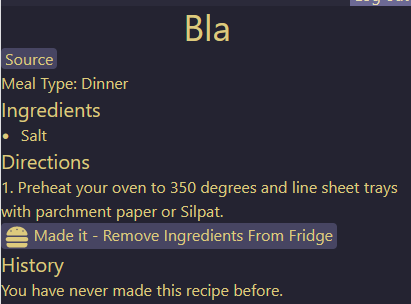
\includegraphics{figures/bad_recipe_entry.png}
\end{figure}

A possible solution for this issue would have been to further pre-process the
data beyond what is discussed in section \ref{sec:data_pre_process} to remove
these entries.\todo{Source}

\subsection{Similar Recipes}
\todo{Similar Recipes}

As recipe similarity only takes the name into account, it is unable to find similarities
in other areas such as ingredient list or directions. An alternative approach to using
recipe names could have been to take the ingredients and directions of the recipe into account,
similar to the strategy used by Freyne and Berkovsky.~\cite{freyne_intelligent_2010}

\subsubsection{Recipe Search}
\todo{Recipe search, based on same model as similar}

\subsection{Meal Type Prediction}
\todo{Meal type prediction}

\todoinline{
    The final part of is the presentation of your results. You may have quantitative or qualitative data, or even both. The best way of presenting your results will be determined
    by the type of data and the nature of your investigation but will usually involve summarising the data in some way.  Data analysis is too large and varied a topic to discuss
    in detail here, and how you do it will be very dependent on the project that you are doing. You are likely to have found out about appropriate methods as part of your
    project. In some cases, it may be appropriate to present calculations, e.g. to demonstrate how performance figures are derived. If you are doing statistical analyses,
    it will be helpful include levels of significance with the results where applicable. The presentation of qualitative data may involve summarising it, identifying significant
    factors, including representative examples, discussing interesting cases or critical incidents in depth, the use of quotations and illustrations, or identifying significant
    categories of content from textual data and looking at how often they occur.  For example, if you had been interviewing people about their use of information, you might
    identify categories related to the type of information, the method of access, etc.
    It may be helpful to use diagrams, charts or tables to present the work or the results. These should come with enough explanation for the reader to make sense of what
    you are showing.

    In general, raw data in the body of your report will be limited to small elements or examples that that you are discussing. Further data can go in your appendices or
    (if bulky) on your OneDrive folder, and you should tell the reader where to look for it. Identifiable personal data should never be included in any part of your submission.
    If you need to refer to individuals, you can mention ‘Participant A’ in your study, or in organisational settings it may be appropriate to refer to someone by their job title.
}

\todo{Results}
